\section{Proposta}

A abordagem principal da proposta está composta por 3 etapas, em alusão ao que se observa no mercado de trabalho. Foram utilizados 2 agentes especializados para atuarem como o Engenheiro de Requisitos da aplicação e o Engenheiro de Software, tendo como papel de PO o usuário que está orquestrando-os \cite{ribeiro_software_2025}.

O primeiro agente utilizou o modelo GPT-5.5, sendo responsável pelo refinamento e detalhamento dos requisitos passados pelo usuário \cite{pires_prompts_2025}. Seu objetivo foi transformar descrições informais de funcionalidade em especificações detalhadas e estruturadas no formato de prompts, para serem utilizadas na etapa de desenvolvimento.

O segundo agente foi responsável por pensar na implementação a partir da descrição detalhada dos requisitos. Sua execução foi feita a partir da plataforma visual OpenCode, utilizando o modelo Mimo 2.5. Esse agente, por sua vez, implementou as funcionalidades solicitadas, realizando a criação ou edição do código-fonte da aplicação e produzindo os artefatos necessários para atender aos requisitos definidos.

Desse modo, o fluxo proposto se baseia nas responsabilidades reais do mercado de trabalho, buscando reproduzir a divisão de responsabilidades observada em equipes de desenvolvimento de software. No entanto, faz-se necessário o conhecimento em programação para entender e especificar para a LLM de geração de requisitos a proposta de segurança, as bibliotecas utilizadas e os meios para alcançar tais objetivos.

\begin{figure}
  \centering
  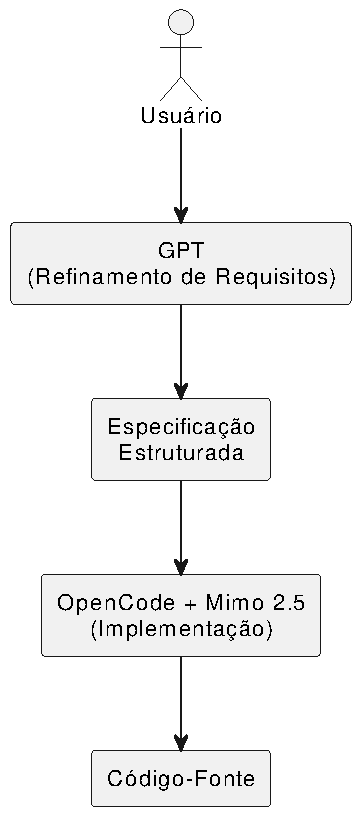
\includegraphics[width=1\linewidth,height=7.5cm,keepaspectratio]{imagens/fluxo-llm}
  \caption{Pipeline de desenvolvimento orientado por agentes para refinamento de requisitos e implementação de software}
  \Description{Fluxo de trabalho entre agentes}
\end{figure}

O agente refinador tem como objetivo transformar solicitações informais e com baixa aceitação pelas LLMs geradoras de código em estruturas mais detalhadas e específicas, auxiliando o desenvolvimento assistido por IA \cite{palermo_agentes_2026}. Para isso, uma descrição textual elaborada, identificando todos os objetivos de uma funcionalidade, regras de negócio, fluxos principais e critérios de aceite, deve ser passada para o modelo utilizado no refinamento \cite{ciudrowski2026explorando}. A LLM é capaz de identificar especificamente pontos de ambiguidade, omissão e inconsistências, aumentando a precisão dos requisitos refinados \cite{palermo_agentes_2026}.

Todos os textos devolvidos pelo modelo de refinação devem ser validados e interpretados para garantir o entendimento completo da funcionalidade, evitando que ela seja desenvolvida de forma incompleta ou incorreta \cite{tolio_llms_2026}. Um ponto de destaque é a importância de existir um profissional técnico por trás da criação desse texto inicial, para conduzir o refinamento orientando as bibliotecas usadas, as validações necessárias e outros pontos que podem impactar o desenvolvimento e a segurança do projeto \cite{ciudrowski2026explorando, palermo_agentes_2026}.

Nesse caso empírico, a escolha pela utilização do GPT se deu pela sua alta capacidade criativa e de escrita, se mostrando extremamente habilidoso no estruturação dos prompts \cite{minaee_large_2024}. Entretanto, entende-se que qualquer agente capaz de escrever prompts com qualidade pode ser usado nessa etapa de desenvolvimento.

Após o refinamento dos requisitos e especificações de implementação, o prompt gerado deve ser utilizado como entrada para o agente de desenvolvimento, utilizando o modo \textit{thinking} para que ocorra o pensamento e a criação do fluxo das tarefas refinadas pela outra LLM. A partir desse momento, o agente poderá efetuar questionamentos ao desenvolvedor, e esses devem ser analisados e respondidos conforme a necessidade do projeto \cite{minaee_large_2024}.

Todos os retornos de código devem ser analisados e verificados por um desenvolvedor com capacidade crítica de entender se o que foi feito possui manutenibilidade, confiabilidade e segurança \cite{ciudrowski2026explorando, palermo_agentes_2026}. As implementações devem seguir o padrão no qual seriam feitas pelo próprio desenvolvedor; com isso, ele deve ter total domínio da linguagem de programação utilizada para compreender a estrutura criada.

Um ponto de destaque é a importância de um arquivo com instruções para o agente se tornar mais técnico e específico no projeto, podendo ser um \textit{AGENTS.md} na raiz, especificando toda a arquitetura do projeto para que ele siga os padrões pré-definidos. O guia de arquitetura, funcionalidades, cores e skills utilizadas dentro desse arquivo funcionará como um manual de instruções para ele se basear e entender como deve estruturar as funcionalidades. Contudo, esse manual deve ser novamente refinado com um modelo de inteligência artificial generativo para deixá-lo descritivo e claro.

Dentro do projeto do editor em \LaTeX{}, foi proposta a utilização da ferramenta open-source OpenCode com o Mimo 2.5, por conta do seu baixo consumo de tokens e da capacidade de pensamento avançado disponível como opção antes da execução do desenvolvimento. Entretanto, é possível se utilizar de outras ferramentas e modelos para essa técnica, tendo em vista a necessidade de um desenvolvedor experiente e com conhecimento na área para tomar a decisão de qual utilizar no projeto.

Para avaliar a aplicabilidade da metodologia proposta, foi desenvolvida uma ferramenta de edição de textos acadêmicos. A ferramenta tem como objetivo auxiliar o processo de escrita, organização e revisão de documentos, integrando recursos tradicionais de edição com funcionalidades baseadas em inteligência artificial. As principais funcionalidades implementadas foram:

\begin{itemize}
    \item Criação, importação e clonagem de projetos a partir de repositórios Git;

    \item Listagem e gerenciamento dos projetos criados pelo usuário;

    \item Interface gráfica para edição de arquivos \texttt{.tex}, contendo recursos de leitura e manipulação do código-fonte;

    \item Criação, edição e organização de subpastas e arquivos dentro do projeto;

    \item Importação e gerenciamento de imagens utilizadas na composição dos documentos;

    \item Reorganização de arquivos e diretórios por meio de operações de arrastar e soltar (\textit{drag and drop});

    \item Visualização do PDF compilado diretamente na aplicação;

    \item Navegação por seções do documento, permitindo acesso rápido a capítulos e subseções por meio de âncoras;

    \item Download do documento PDF gerado;

    \item Inicialização de repositórios Git nos projetos e execução de comandos básicos de versionamento (em fase de aprimoramento para correção de inconsistências);

    \item Apresentação de mensagens de erro detalhadas durante o processo de compilação, facilitando a identificação e resolução de problemas;

    \item Integração com modelos de inteligência artificial para auxílio na revisão textual, incluindo correção ortográfica, análise de concordância verbal, melhoria de sentenças e identificação de repetição excessiva de termos. Foram utilizados modelos locais baseados em Llama e modelos disponibilizados pela plataforma Groq, permitindo que o usuário selecione o provedor desejado por meio de variáveis de ambiente;

    \item Desenvolvimento da documentação técnica do projeto utilizando a ferramenta MkDocs;

    \item Implementação de pipeline de integração e entrega contínua (CI/CD) para geração e publicação automática da documentação via GitHub Pages após alterações no repositório principal.
\end{itemize}

Como trabalhos futuros e itens presentes no backlog de desenvolvimento, destacam-se:

\begin{itemize}
    \item Implementação de uma análise completa do projeto utilizando inteligência artificial para identificar e sugerir correções ortográficas e gramaticais em todos os arquivos do documento, sem depender do arquivo atualmente aberto pelo usuário;

    \item Utilização de inteligência artificial para avaliar a aderência do conteúdo desenvolvido aos requisitos definidos pela banca avaliadora, identificando possíveis lacunas ou melhorias necessárias;

    \item Desenvolvimento de um recurso de assistência ao usuário para esclarecer dúvidas relacionadas à utilização de recursos \LaTeX, incluindo auxílio na aplicação de comandos de formatação textual, como negrito, itálico e outros elementos de estruturação do documento.
\end{itemize}

A Figura~\ref{fig:layout-sistema} apresenta o layout por dentro da ferramenta desenvolvida para apoiar a elaboração de textos acadêmicos em \LaTeX. A aplicação foi projetada para integrar, em um único ambiente, recursos como organização de documentos e assistência baseada em inteligência artificial.

Na interface, é possível observar a estrutura de arquivos do projeto, permitindo a navegação entre seções, imagens, referências bibliográficas e demais artefatos que compõem o documento. Foi utilizado o modelo padrão da conferência para exemplificar como seria um texto produzido por ele, além de ser testado de forma prática na construção desse artigo. 

A área central é destinada à edição do conteúdo em \LaTeX, enquanto o painel lateral exibe a visualização do PDF gerado em tempo real, possibilitando ao usuário acompanhar imediatamente os resultados das alterações realizadas.

Além das funcionalidades tradicionais de edição, a ferramenta incorpora recursos voltados a assistentes de IA para apoiar na escrita, refinamento de conhecimento e, em versões futuras, auxílio na utilização de comandos \LaTeX. Integrações com plataformas como GitHub também podem ser observadas na imagem, facilitando o gerenciamento e versionamento do projeto, facilitando a escrita em conjunto. Também é possível visualizar a navegação por sumário e exportação do documento em formato PDF, concentrando em uma única plataforma os principais recursos necessários para a produção de trabalhos acadêmicos.

A solução foi desenvolvida seguindo uma arquitetura de monolito modular, utilizando React no frontend e Express no backend. Para simplificar o processo de configuração do ambiente, diminuindo a dificuldade inicial em sua utilização, a infraestrutura é disponibilizada por meio de contêineres Docker, eliminando a necessidade de instalação manual de dependências e bibliotecas por parte dos usuários. Dessa forma, a ferramenta reduz o esforço inicial de configuração e permite que pesquisadores e estudantes concentrem suas atividades na produção do conteúdo acadêmico.

\begin{figure}[htbp]
  \centering
  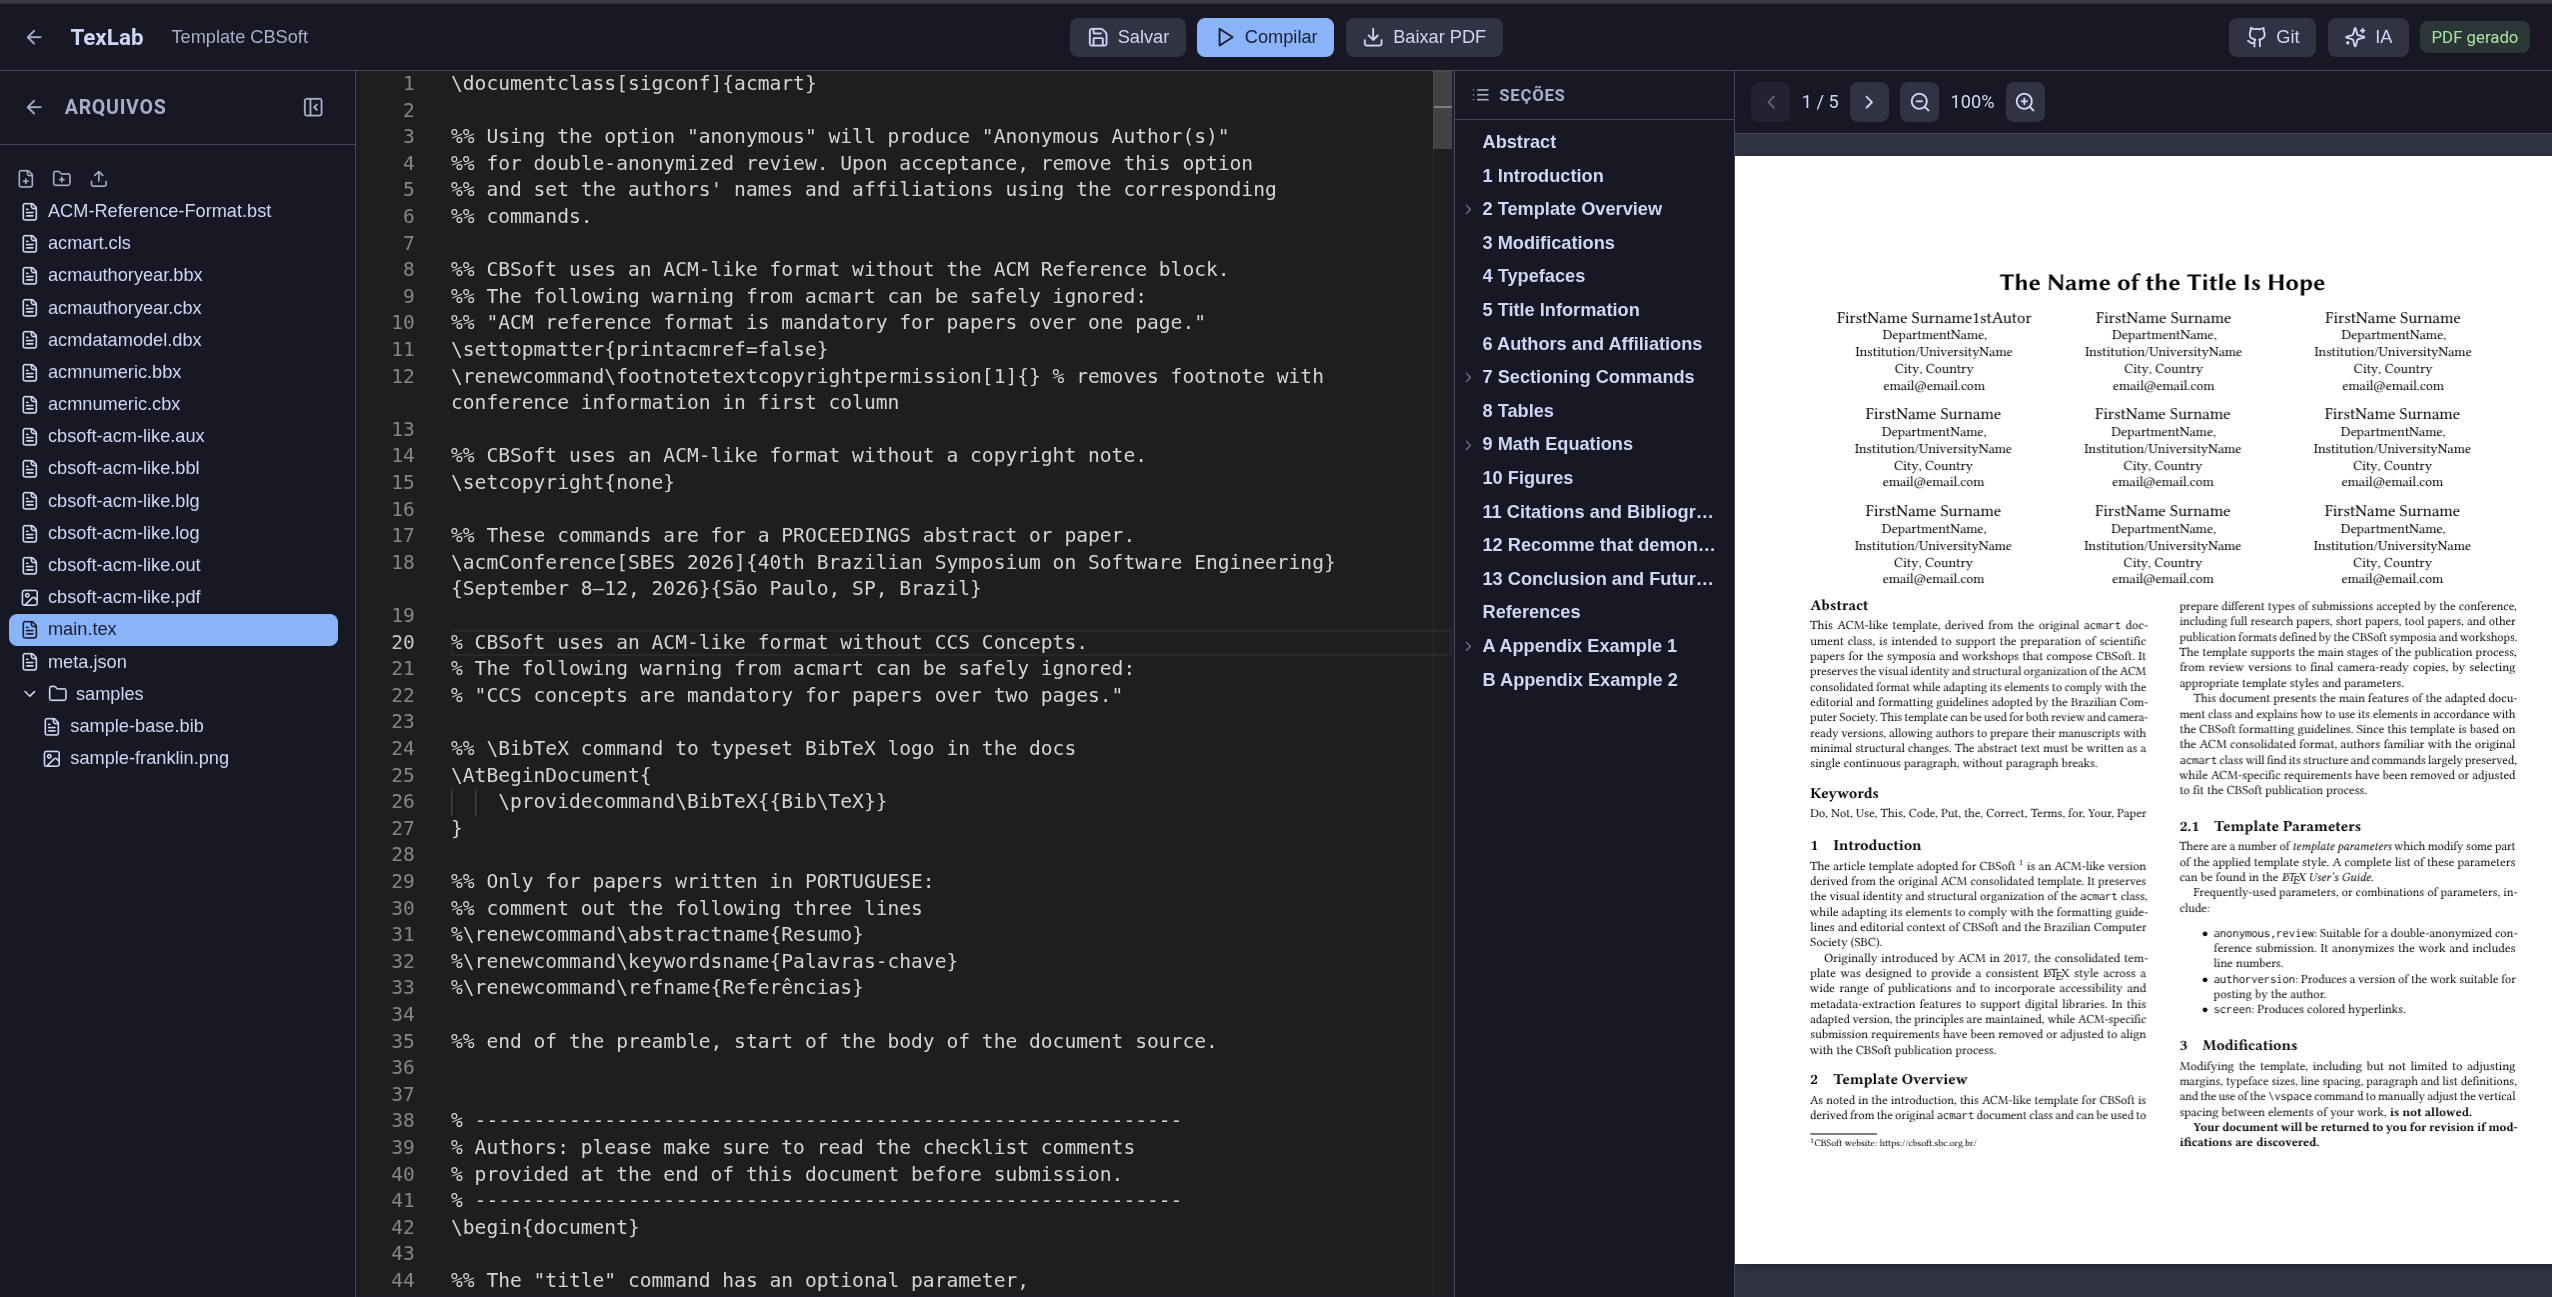
\includegraphics[width=\linewidth,keepaspectratio]{imagens/layout-texlab}
  \caption{Layout do sistema de edição de textos em \LaTeX.}
  \label{fig:layout-sistema}
  \Description{Layout do sistema}
\end{figure}

Durante o processo de desenvolvimento da ferramenta, foi observado que a utilização de uma LLM para realização do refinamento e criação do prompt contribuiu de forma positiva com os resultados. Ela auxiliou na robustez do prompt, consolidando a ideia, adicionando regras de negócio e requisitos não funcionais. Com isso, diminuiu a ambiguidade, inconsistências e melhorou a comunicação com o agente de desenvolvimento.

Funcionalidades simples puderam ser implementadas com um único prompt ou com poucas interações adicionais. Enquanto isso, funcionalidades mais complexas demandaram ciclos extras de desenvolvimento assistido pelo agente, sendo necessário testar a aplicação e entender onde não estava funcionando para explicar para o agente refinar um texto de melhoria.

A análise feita demonstrou a importância de um profissional técnico por trás para manusear a ferramenta durante o processo, conduzindo o modelo a produzir código com alta qualidade. Dessa forma, a metodologia não substitui o papel do desenvolvedor, mas busca ampliar sua produtividade por meio da automação de atividades de especificação e implementação.

Por fim, observou-se que a disponibilização de documentos de contexto, como o arquivo AGENTS.md contendo informações sobre arquitetura, convenções, padrões de layout e tecnologias utilizadas, contribuiu para aumentar a aderência das implementações aos padrões previamente definidos para o projeto.